% !TeX spellcheck = en_GB
\documentclass[12pt]{article}

\usepackage[a4paper, margin=0.7in]{geometry}
\usepackage{algorithm,algpseudocode}
\usepackage{caption}
\usepackage{algpseudocode}
\usepackage{graphicx}
\usepackage{verbatim}
\usepackage{comment}
\usepackage{amsmath}
\usepackage{amssymb}

\newtheorem{theorem}{Theorem}
\newtheorem{proposition}[theorem]{Proposition}
\newtheorem{lemma}[theorem]{Lemma}
\newtheorem{proof}[theorem]{Proof}

\begin{document}
\title{An Efficient Recursive Approach for Workload Distribution on Heterogeneous Systems}
\author{Hamidreza Khaleghzadeh}
\date{26 Jan 2017}

\maketitle

\section{Introduction}
In this report, we propose a new method called \textit{WorkPart} which benefits from Branch-and-Bound programming technique to find the optimal workload distribution on $p$ heterogeneous processors so that the parallel execution time is minimized. We will explain the proposed approach in this report.

\section{Formulation of Performance Optimization Problem}
Consider a workload of size $n$ executed using $p$ heterogeneous processors. Let time functions of processors be represented by set $T$ where $T_i=\{(x_i^0,t_i(x_i^0)),(x_i^1,t_i(x_i^1)),\cdots,\allowbreak (x_i^{m-1},t_i(x_i^{m-1}))\}$, $0 \le i \le p-1$, $m \in \mathbb{Z}_{>0}$. There is one time function per each processor where $T_i$ represents the time function of the processor $P_i$ which is represented by a discrete set of experimental data points separated by minimum granularity, $\Delta x$. A given data point $(x,t(x))$ determines a workload with size of $x$ along with its execution time ($t(x)$). It should be noted that the workload with size of $n$ should be a multiple of $\Delta x$. The problem, $WorkPart(n,p,T,t_{opt},D_{opt})$, is to find a partitioning, $D_{opt} = <x_{opt}^0,\cdots,x_{opt}^{p-1}>$, of the workload of size $n$ among $p$ processors that minimizes the parallel computation time of the workload ($t_{opt}$). The parameters of $(n,p,T)$ and $(t_{opt},D_{opt})$ are the inputs and outputs of the problem, respectively. The problem can be formulated as following:
\begin{equation} \label{eq1}
\begin{split}
t_{opt} = minimize \quad \max_{i=0}^{p-1} \quad t_i(x^i) \\
\text{Subject to } x^0+x^1+\cdots+x^{p-1} = n \\
0 \le x^i \le n \qquad i = 0,\cdots,p-1 \\
\text{Where } p,n,x^i \in \mathbb{Z}_{>0} \text{ and } t_i(x^i) \in \mathbb{R}_{>0}.
\end{split}
\end{equation}

It is noteworthy that if a given $x^i$ is equal with 0, no problem is assigned to $P_i$. Therefore, the number of selected processors in the optimal workload distribution may be less than $p$.

\section{An Example}
In this section, using a simple example, we will explain how the problem $WorkPart$ is solved by the proposed algorithm called $HetWD$ which is responsible to find optimal distribution. Let a workload size of $n = 16$ runs on $p = 4$ processors with time functions $T=\{T_0,\cdots,T_3\}$. Assume, for the sake of simplicity, the minimum granularity is 1 ($\Delta x = 1$). 

Figure \ref{ex_fig1} illustrates time functions sorted in non-decreasing order of time. Each cell in time functions shows execution time and its label is the problem size. To restrict the search area, the algorithm applies a time threshold represented by $t_{opt}$. All data points with greater or equal execution time than the time threshold are ignored. During the initialization step of the algorithm, the time threshold is set to load-equal execution time. According to the load-equal distribution, the assigned problem size to each processor should be $\frac{16}{4}=4$ where its parallel execution time is $\max_{i=0}^{3} t_i(4) = \max \{12,6,4,4\} = 12$. All data points with smaller execution time of 12 consist our search area highlighted in time functions (Figure \ref{ex_fig1}).

In the figure, there is a matrix called $Mem$ so that rows $Mem[1]$ and $Mem[2]$ store intermediate results for processors $P_1$ and $P_2$ (one row per processor). Each row in $Mem$ consists of 17 compound cells ($=16+1$) where $Mem[i][w]$, $i \in \mathbb{Z}_{[1,2]}, w \in \mathbb{Z}_{[0,n]}$ holds some information about distribution of work-size of $w$ on $P_i$ such as:

\begin{itemize}
	\item \textbf{$Mem[i][w].eTime$:} Parallel execution time of $w$ on $P_i,\cdots,P_{p-1}$,
	\item \textbf{$Mem[i][w].lastIndex$:} The index of last evaluated data point in the time function $T_i$. In case a memory cell stores the optimal result, it is labelled as $Finalized$ and $Mem[i][w].lastIndex = \_FI$.
	\item \textbf{$Mem[i][w].size$:} The problem size assigned to $P_i$ along with its execution time
	\item \textbf{$Mem[i][w].time$:} The execution time of the assigned partition to $P_i$ ($t_i(Mem[i][w].size)$).
	
\end{itemize}

The matrix is empty at the beginning of the algorithm.

\begin{figure}[!t]
	\centering
	\fbox{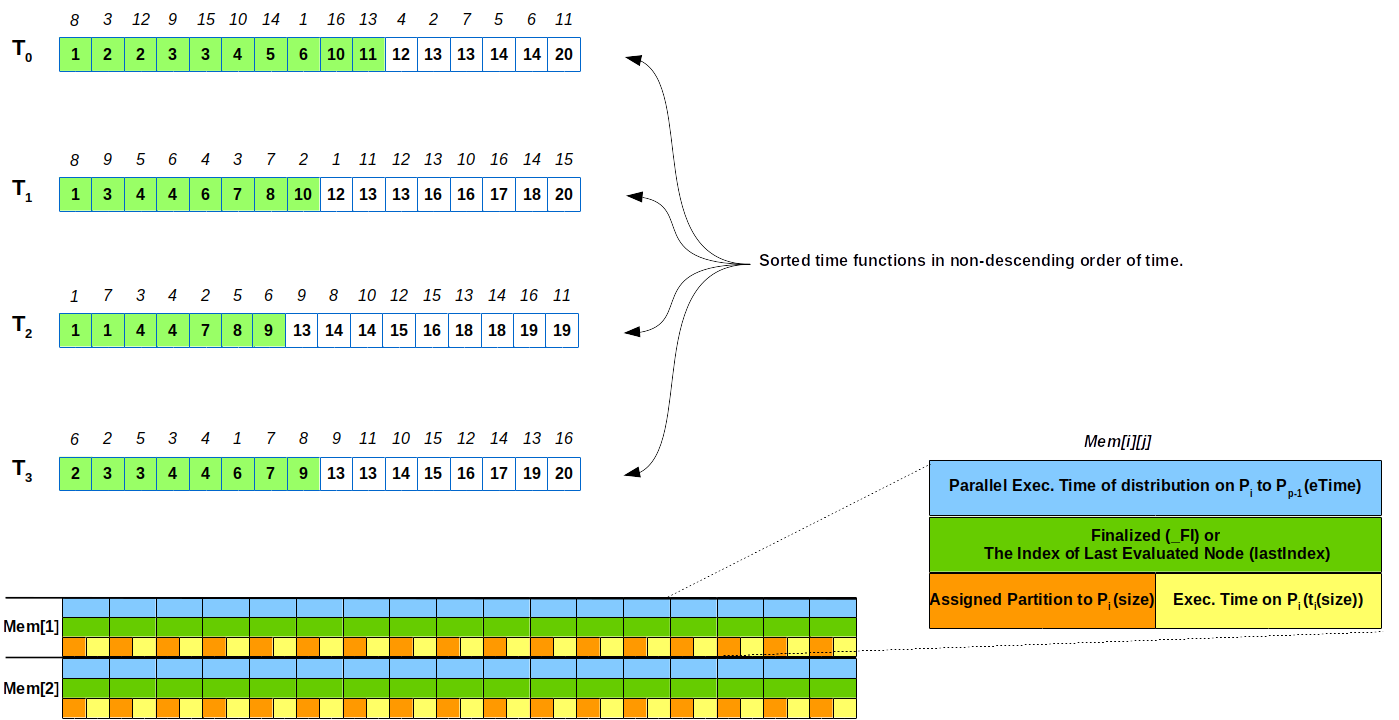
\includegraphics[width=\textwidth,height=\textheight,keepaspectratio]{Images/example/fig1.png}}
	\caption{Data structures and applying time threshold to restrict search area}
	\label{ex_fig1}
\end{figure}

To find optimal solution, all possible distributions should be evaluated. To this end, the method uses Branch-and-Bound technique which finds the optimal solution using in-depth tree traverse. Figure \ref{ex_fig2} shows the search tree built and traversed by $HetWD$ for finding the optimal workload distribution. There are two values associated with each node. Suppose node $X/Y$ on the level $L_{i \in \mathbb{Z}_{[0,\cdots,p - 1]}}$ where $X$ is remaining workload should be distributed, and $Y$ is a size threshold which is maximum possible work-size can be distributed on processors $P_i$ to $P_{p-1}$. According to the time functions, the maximum workload size with execution times less than 12 are 16, 9, 6 and 8 for $T_0,\cdots,T_3$, respectively. As shown in the figure, size thresholds are as following: for the level $L_0$ is $16+9+6+8=40$, for $L_1$ is $9+6+8=24$, for $L_2$ is $9+6=15$ and for $L_3$ is 8. In addition, the pair assigned to the edge on level $L_{i}$ determines assigned work-size to the processor $P_i$ and its corresponding execution time, respectively. If the edge label of a given level $L_{i \in \mathbb{Z}_[0,p-1]}$ is $0,0$, it means that no workload is assigned to $P_i$. 

Each level in the tree is responsible for one processor to examine all data points existing in its time function from the first to the last elements which have less execution time than time threshold. Let's take a look at figure \ref{ex_fig2}. Before examination of data points existing in time functions, zero problem sizes are assigned to processors $P_0$ and $P_1$. Thus the remaining work-size should be distributed on $P_2$ and $P_3$ is still 16. But, since the remaining size (16) is greater than the size threshold of $L_2$, the node 16/15 will not be extended more and cut.

\begin{figure}[!t]
	\centering
	\fbox{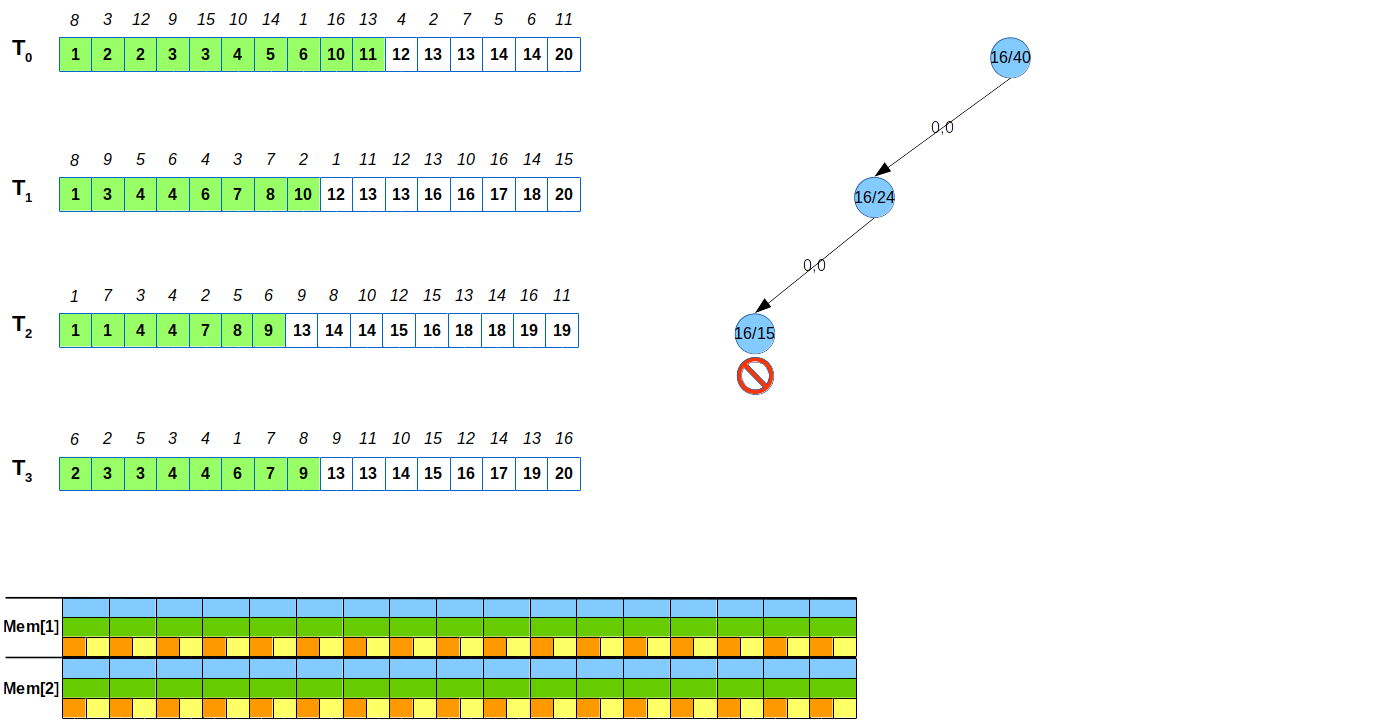
\includegraphics[width=\textwidth,height=\textheight,keepaspectratio]{Images/example/fig2.png}}
	\caption{Using size thresholds for cutting branches}
	\label{ex_fig2}
\end{figure}

Figure \ref{ex_fig3} depicts a solution found with parallel execution time of 9. The partitions assigned to processors $P_0$ to $P_3$ are $D_{opt}=<0,8,0,8>$, respectively.

Having found a solution, $HetWD$ are required to perform some post-solution operations as follows:
\begin{enumerate}
	\item updating time threshold ($t_{opt}$)
	\item updating size thresholds
	\item memorizing the current solution into $Mem$
	\item finding the uppermost node in the tree with maximum execution time and backtracking to its ancestor.
\end{enumerate}

In this example, $t_{opt}$ is updated to 9. As shown in the figure, the search area highlighted in each time function is also reduced due to the new $t_{opt}$. Once the green search area is shrunk, then size thresholds are recalculated. New size thresholds are replaced with $\{38,23,14,7\}$ (figure \ref{ex_fig4}). In addition, we are required to store the intermediate solutions in $Mem$. To this end, the solution found for the workload sizes on $P_1$ and $P_2$ should be stored. If the solution path from the root to the leaf is traced in the figure \ref{ex_fig3}, the problem size for $P_1$ and $P_2$ are respectively 8 and 16. Therefore, $Mem[2][8]$ and $Mem[1][16]$ has been updated to store these intermediate solutions. 

\begin{figure}[!t]
	\centering
	\fbox{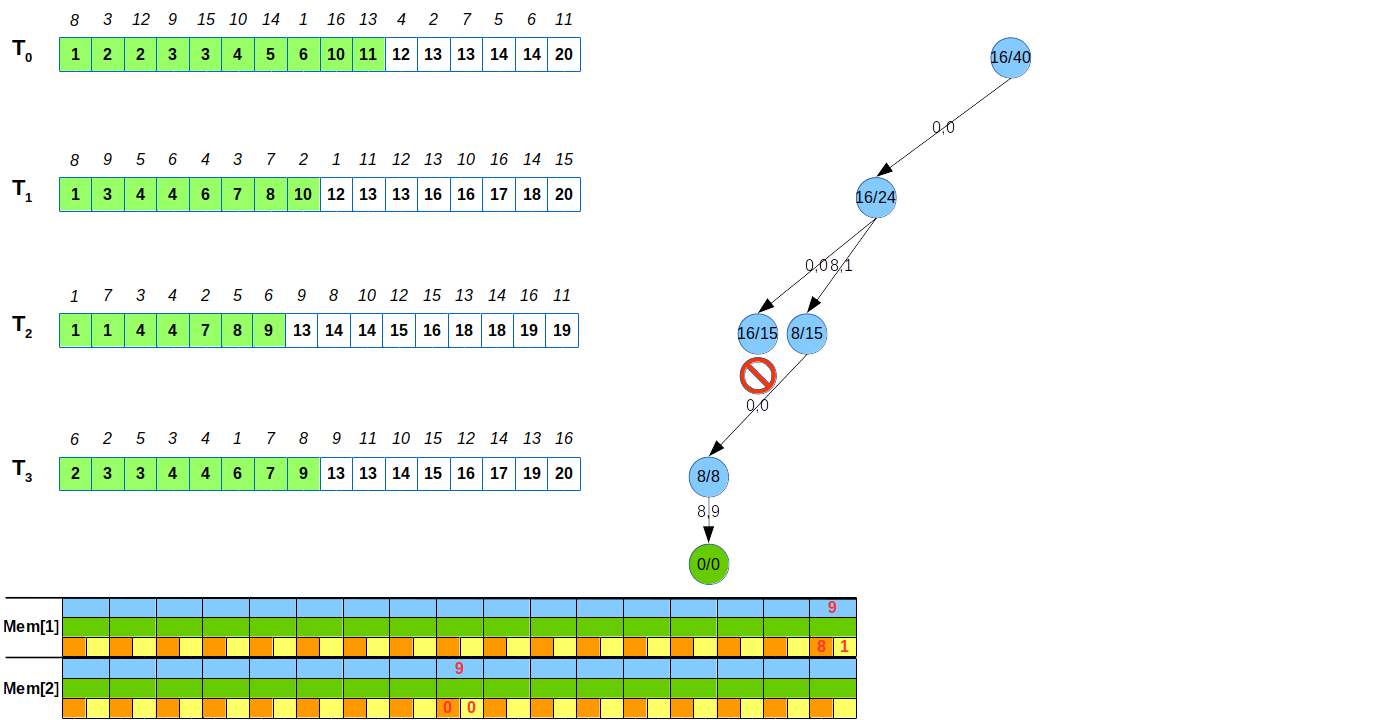
\includegraphics[width=\textwidth,height=\textheight,keepaspectratio]{Images/example/fig3.png}}
	\caption{Finding a solution an its post-solution operations}
	\label{ex_fig3}
\end{figure}

The algorithm keeps on examination of more data points. Figure \ref{ex_fig4} illustrates new solution with better computation time of 7. All post-solution operations should again be performed. As time threshold decreases to 7, new size thresholds will be $\{37,22,13,6\}$ (figure \ref{ex_fig5}). In addition, $Mem[2][8]$ and $Mem[1][16]$ are updated (figure \ref{ex_fig4}).

\begin{figure}[!t]
	\centering
	\fbox{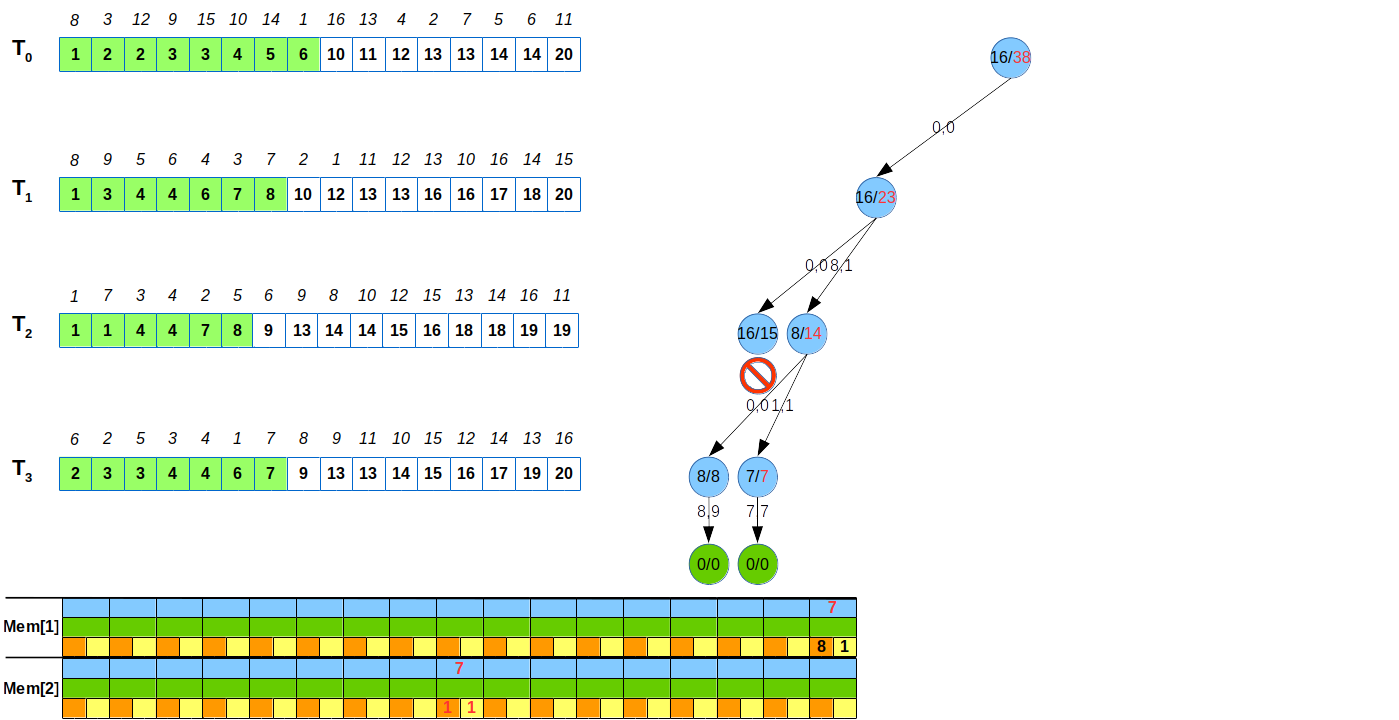
\includegraphics[width=\textwidth,height=\textheight,keepaspectratio]{Images/example/fig4.png}}
	\caption{Converging to the optimal solution}
	\label{ex_fig4}
\end{figure}

In figure \ref{ex_fig5}, the parallel execution time is 4, and the maximum time occurs at level $L_2$. Since we are looking for a new solution with the execution time less than 4, more expansion of node 8/13 makes no sense. Because of non-decreasing order of execution time in time functions, following data points in the time function $T_2$ do not have less execution time than $t_{opt}$. It means that more expanding of this node would not bring a better distribution with an execution time less than 4. So, we backtrack to its ancestor in level $L_1$. Since there is no better solution than $t_{opt}=4$ for workload size of 8 on $P_2$ and $P_3$, $Mem[2][8]$ is finalized in (Labelled as $\_FI$).

\begin{figure}[!t]
	\centering
	\fbox{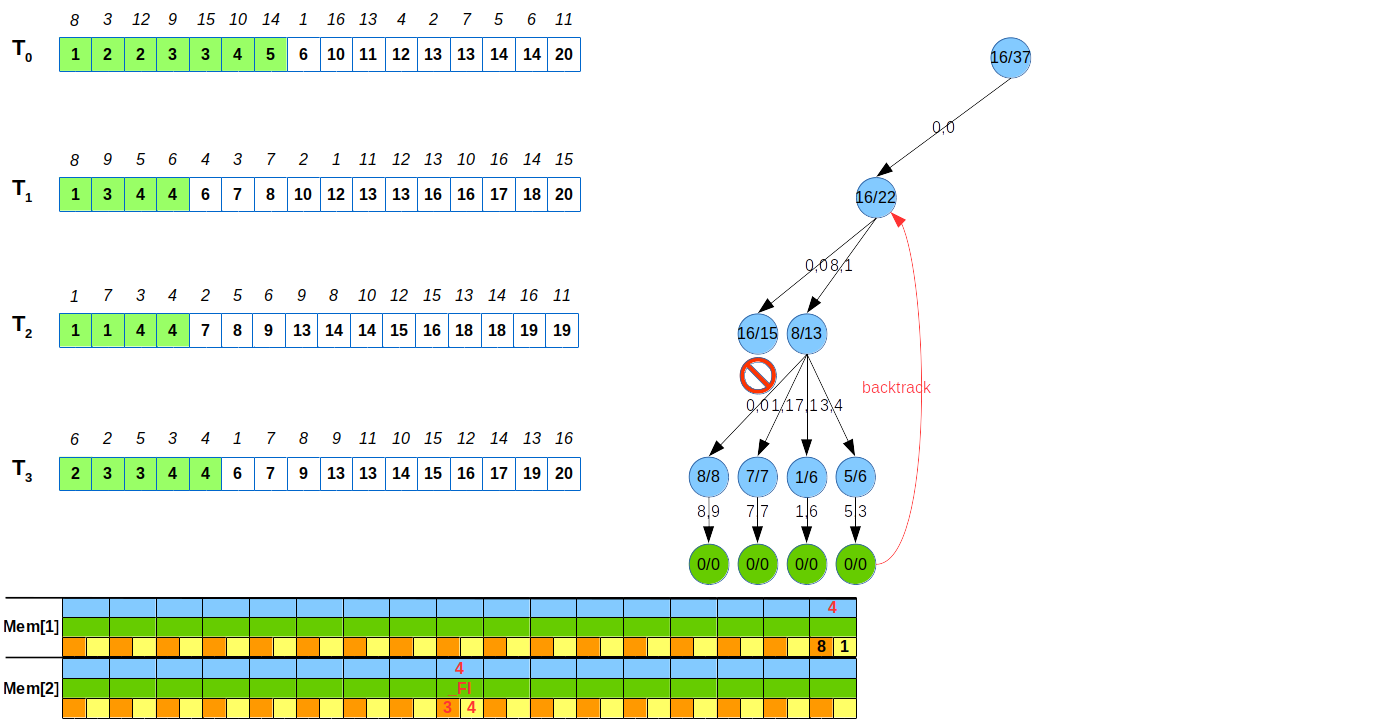
\includegraphics[width=\textwidth,height=\textheight,keepaspectratio]{Images/example/fig5.png}}
	\caption{Backtracking}
	\label{ex_fig5}
\end{figure}

Having backtracked, the process continues from level $L_1$. Figure \ref{ex_fig6} shows this step. The algorithm selects (9,3) from $T_1$. Its expansion results in a solution with better execution time. Thus, all post-solution operations are done after finding a solution are applied where $t_{opt}$ decreases to 3, and $Mem[2][7]$ and $Mem[1][16]$ are updated. It is noteworthy that the last index examined in $T_2$ is stored in $Mem[2][7].lastIndex$. For instance, suppose that we again want to find a distribution for workload 7 on $P_2$ and $P_3$. In this case, we will not be required to start from the beginning of the time function $T_2$. Having restored the last stored solution for work-size 7, the process is resumed from the node with index 1.

\begin{figure}[!t]
	\centering
	\fbox{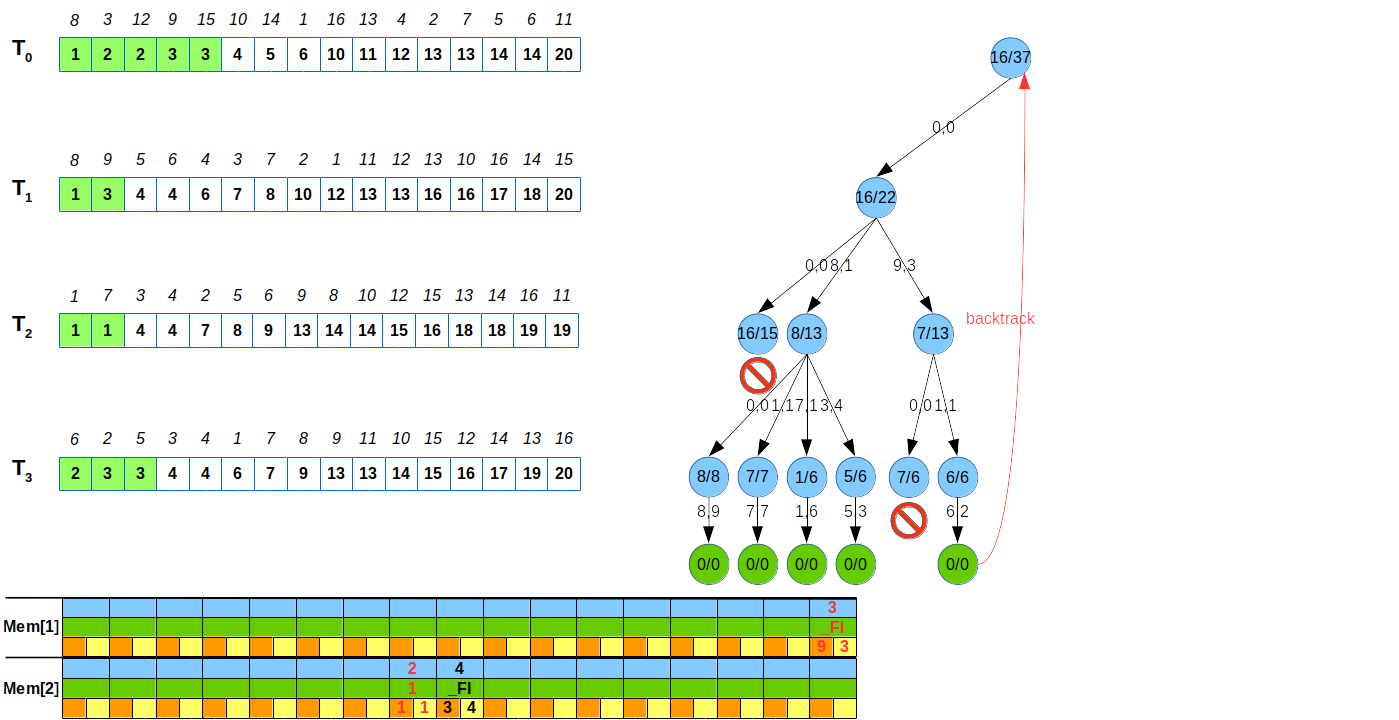
\includegraphics[width=\textwidth,height=\textheight,keepaspectratio]{Images/example/fig6.png}}
	\caption{Storing last evaluated index in Mem for resuming the process from where was interrupted}
	\label{ex_fig6}
\end{figure}

After backtracking to the root, the algorithm again needs to find a solution for workload with size of 8 on $P_2$ (Node 8/13 in figure \ref{ex_fig7}). Since the problem for this workload on $P_2$ has already been solved, we are not required to resolve it from scratch. Instead, the solution can be retrieved from $Mem$. The stored solution is finalized and it can be used to make final decision. It should be mentioned that if it is not finalized, we are required to extract the previous stored solution and then resume the process from where it was interrupted using the stored index in the memory.

In this example, using the memory, we extract the distribution of work-size 8 on $P_2$ and $P_3$. Since its parallel execution time is greater than current one, this solution is ignored.

\begin{figure}[!t]
	\centering
	\fbox{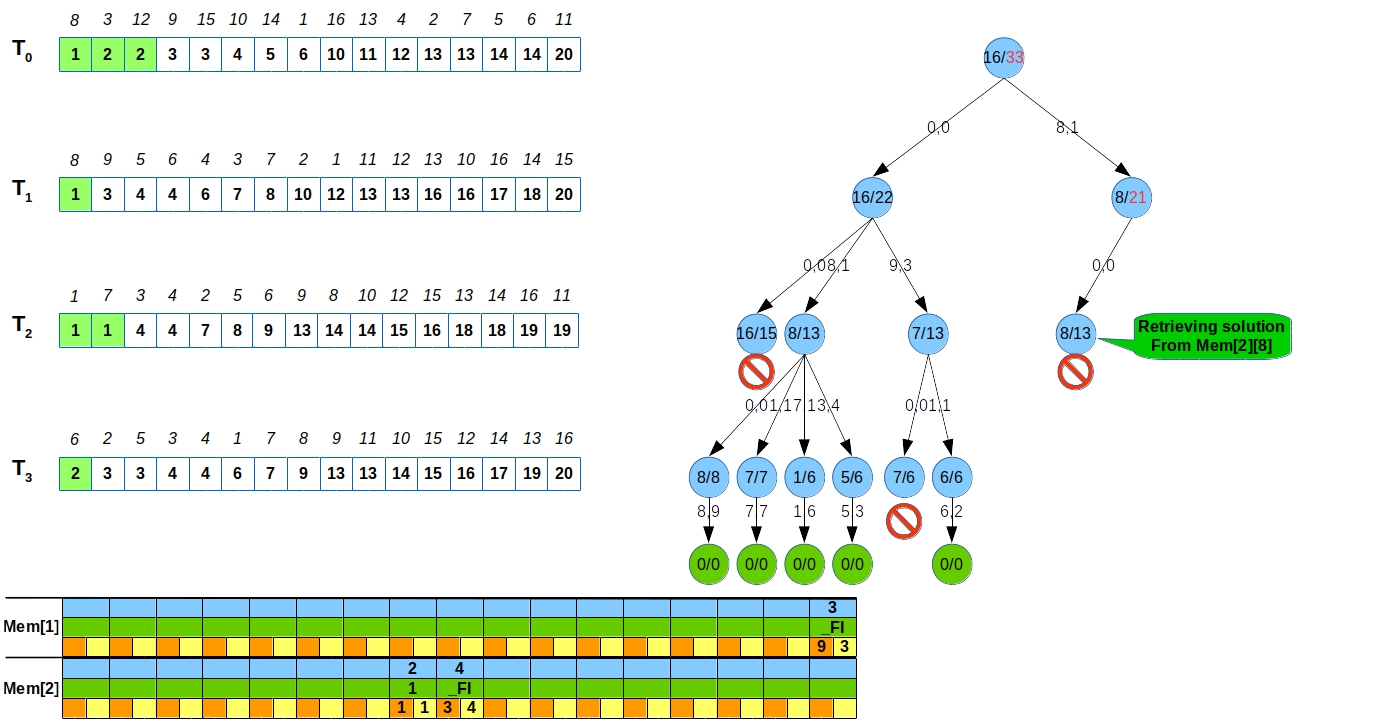
\includegraphics[width=\textwidth,height=\textheight,keepaspectratio]{Images/example/fig7.png}}
	\caption{Extracting a sub-solution from Mem}
	\label{ex_fig7}
\end{figure}

Finally, $HetWD$ examines the data point $(8,1)$ from $T_1$ (Figure \ref{ex_fig8}). It finds the solution $D_{opt}=<8,8,0,0>$ with the parallel execution time of 1 ($t_{opt}=1$). Since time threshold is updated with 1, there is no data points remaining to examine and the last distribution in $D_{opt}$ with the parallel execution time $t_{opt}$ is returned as the optimal distribution.

It should be noted that the algorithm returns load-equal workload distribution if it cannot find any solution with less parallel execution time. It happens when there is no distribution with sum to $n$ and less parallel execution time than that of load-equal workload distribution.

\begin{figure}[!t]
	\centering
	\fbox{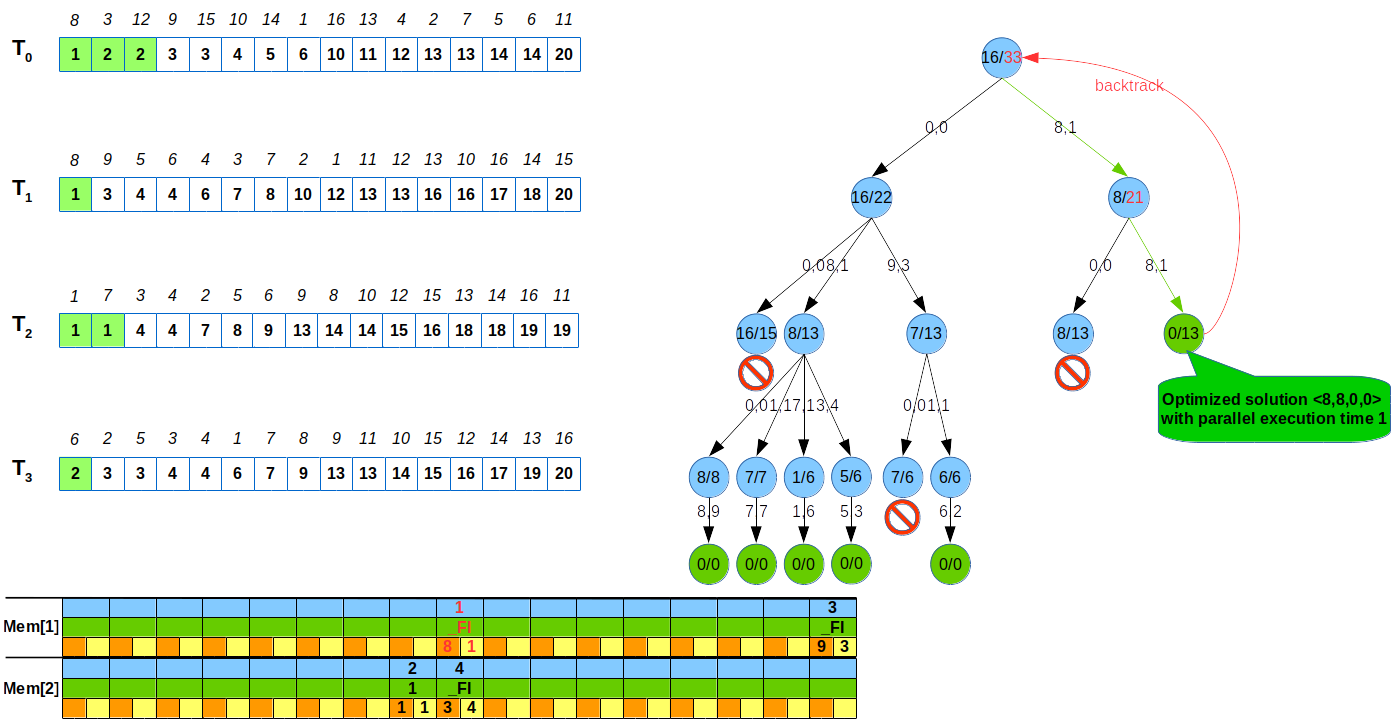
\includegraphics[width=\textwidth,height=\textheight,keepaspectratio]{Images/example/fig8.png}}
	\caption{Finding the optimal solution}
	\label{ex_fig8}
\end{figure}

\section{The Proposed Efficient Algorithm}
In this section, we present an efficient algorithm to solve $WorkPart$ problem (Algorithm \ref{alg1_code}). The inputs to the algorithm are: the workload size, $n$ ($n$ should be a multiple of $\Delta x$), the number of heterogeneous processors, $p$ and a list of $p$ time functions, $T=\{T_0,T_1,\cdots,T_{p-1}\}$. The outputs of the algorithm are the optimal execution time, $t_{opt}$ and the optimal workload distribution, $D_{opt}$. It is noteworthy that the number of processors selected by WorkPart in the optimal workload distribution may be less than $p$.

The function obtains load-equal distribution an initializes $t_{opt}$ and $D_{opt}$. It returns the workload distribution so that $x_{opt}^i=\frac{n}{p}$, $t_{opt}=\max_{j=0}^{p-1} t_i(\frac{n}{p})$, $\forall i \in [0,p-1]$ (Algorithm \ref{alg1_code}, line \ref{alg1_leq}). It is important to note that $\sum_{i=0}^{p-1} x_{opt}^i = n$. 

Array S contains the size thresholds, which is illustrated in the example. IT is a list of sizes where $S_{i \in \mathbb{Z}_{[0..p - 1]}}$ represents the maximum workload size can be distributed on processors $P_i,...,P_{p - 1}$ with maximum parallel execution time of $t_{opt}$. It is the function size\_thresholds responsible for determining these values (Algorithm \ref{alg1_code}, line \ref{alg1_s_th}). There is a two-dimensional matrix with size of $(p-2)*(n+1)$ called $Mem$ to memorize the points that have already been visited during the recursive invocations. The array value $Mem[i][n]$, $\forall i \in [1,p-2]$ contains some information for workload with size of $n$ distributed on processors $P_i,\cdots,p-1$. the information includes: the parallel execution time, the partition assigned to $P_i$ along with its execution time,the index of last examined data point in $T_i$ and the status of memory (Finalized or Not\_Finalized). This memorization ensures that there are only $O(n*m*p)$ recursive invocations of the core function (Algorithm \ref{alg2_code}). Having initialized $Mem$, $WorkPart$ invokes the $HetWD$ to find the optimal workload distribution.

\begin{algorithm}
	\scriptsize
	\caption{Algorithm Finding Optimal workload Distribution of Size $n$ for Maximizing Performance} \label{alg1_code}
	\begin{algorithmic}[1]	
		\Function{WorkPart}{$n, p, T, t_{opt}, D_{opt}$}
		\Statex \textbf{INPUT:}
		\Statex Workload size, $n \in \mathbb Z_{> 0}$
		\Statex Number of processors, $p \in \mathbb Z_{> 0}$
		\Statex Time functions, $T = \{T_0,...,T_{p - 1}\}$. $T_i={(x_i^0,t_i(x_i^0)),\cdots,(x_i^{m-1},t_i(x_i^{m-1}))}, $ $t_i(x_i^0) \le t_i(x_i^1) \le \cdots \le t_i(x_i^{m-1}), $ $x^j \in \mathbb Z_{> 0},$ $\forall j \in [0,m-1],$ $\forall i \in [0,\cdots,p-1]$ 
		\Statex \textbf{OUTPUT:}
		\Statex Optimal execution time, $t_{opt} \in \mathbb R_{> 0}$
		\Statex Optimal workload distribution, $D_{opt} = {x_{opt}^0,...,x_{opt}^{p-1}}, x_{opt}^i \in T_i $ $or 0,$ $\forall i \in [0,\cdots,p-1]$. 
		\Statex
		\State $(t_{opt}, D_{opt})$ $\gets$ \Call{load\_equal\_dist}{$n,p$}	\label{alg1_leq}
		\State $S$ $\gets$ \Call {size\_thresholds}{$T,t_{opt}$}	\label{alg1_s_th}
		\State $\forall i \in [1,\cdots,p-2],$ $j \in [0,\cdots,n]$
		\State \hskip\algorithmicindent $Mem[i][j]$ $\gets$ $(0,0)$
		\State \Call {HetWD}{$n,p,0,T,S,NULL,D_{cur},Mem,t_{opt},D_{opt}$} \label{alg1_hetwdCall}
		\State \Return $(t_{opt},D_{opt})$		
		\EndFunction		
	\end{algorithmic}
\end{algorithm}

\section{Recursive Algorithm $HetWD$} \label{sec_code}
In order workload with size of $n$ to be optimally distributed on $p$ processors, WorkPart invokes a core routine called $HetWD$ (Algorithm \ref{alg1_code} line \ref{alg1_hetwdCall}). This proposed function is responsible to examine possible workload distributions using the Branch-and-Bound technique and find optimal solution. The search area is a tree data structure which is constructed implicitly using Depth First Search (DFS) technique and consists of maximum $p$ levels. Each level belongs to one processor where level $L_0$ to $P_0$ and so on, and all possible partitions can be assigned to a given processor $P_i$ are examined in $L_i$. 

To cut sub-optimal branches, we benefits from some optimizations that will be explained in section \ref{sec_opt}. In addition, we will explain how memorization of intermediate solutions prevent duplicate recalculations (Section \ref{sec_mem}).

$HetWD$ is illustrated in Algorithm \ref{alg2_code}. The while loop (Algorithm\ref{alg2_code}, lines \ref{Alg1_mainLoop1}-\ref{Alg1_mainLoop2}) builds the main section of the algorithm which is responsible for scanning time functions from left to right to examine all data points with execution time less than $t_{opt}$. The current processor which is under processing is represented by $c \in \{P_0,\cdots,P_{p-1}\}$. Selected work-sizes for each processor is stored in $D_{cur}={x^0,\cdots,x^{p-1}}$ where $d^i \in T_i$ determines current selected partition for $P_i$. It is important to note that $D_{opt}={x_{opt}^0,\cdots,x_{opt}^{p-1}}$ holds the best distribution found so far. 

The algorithm goes ahead in depth from $P_0$ (the root of the implicit tree) up to $P_{p-1}$ (a leaf) while $n$ is larger than zero. In each level, it stores current partition in $D_{cur}$. Once a solution is found, Post\_Solution\_Operations is called to perform post-solution activities such as: updating $t_{opt}$, $D_{opt}$, array $S$ and determining to which level the process should backtrack (determined with $bk$).

\begin{algorithm}
\scriptsize
\caption{Pseudocode of recursive workload partitioning on heterogeneous platforms} \label{alg2_code}
\begin{algorithmic}[1]	
\Function{HetWD}{$n, p, c, T, S, bk, D_{cur}, Mem,t_{opt}, D_{opt}$}
\Statex
	\If{$c = p - 1$}	\label{Alg1_leaf1}
		\If{$t_c(n) < t_{opt}$}
			\State $D_{cur}[c]$ $\gets$ $(n,t_c(n))$
			\State \Call{Post\_Solution\_Operations}{$D_{cur},t_{opt},D_{opt},S,bk,Mem$}
		\EndIf
		\State \textbf{return}	
	\EndIf				\label{Alg1_leaf2}
	\State $<size_c,time_c>$ $\gets$ $(0,0)$
	\State $curIndex=-1$
	\If{$c > 0 \wedge c \leq p - 2$}	\label{retrieveMem1}
		\State $<isReturn,curIndex>$ $\gets$ \Call{ReadFromMemory}{$n,p,c,t_{opt},T,bk, D_{cur}$}
		\If{$isReturn=true$}
			\State \textbf{return}
		\Else
			\State $<size_c,time_c>$ $\gets$ $(x_c^{curIndex},t_c(x_c^{curIndex}))$
		\EndIf
	\EndIf							\label{retrieveMem2}
	\While{$time_c < t_{opt}$} \label{Alg1_mainLoop1}
		\If{$n = size_c \vee n > size_c \wedge S[c + 1] \geq (n - size_c)$}	\label{Alg1_non_leaf1}
			\State $D_{cur}[c]$ $\gets$ $(size_c, time_c)$
			\If{$n = size_c$}			
				\State \Call{Post\_Solution\_Operations}{$D_{cur},t_{opt},D_{opt},S,bk,Mem$}
			\Else
				\State \Call{HetWD}{$n-size_c,p,c+1,t_{opt},T,S,bk,D_{cur}$}	\label{Alg1_recall}
			\EndIf
			\If{$bk < c$}
				\If{$t_c(x_c^{curIndex})=t_{opt}$}	
					\State $Mem[c][n].$\Call{makeFinal}{ }
				\Else
					\State $Mem[c][n].last_{index} = curIndex$ \label{alg1_lastIndex}
				\EndIf		
				\State \textbf{return}
			\ElsIf{$bk = c$}
				\State $bk = NULL$
				\State $Mem[c][n].$\Call{makeFinal}{ }
				\State \textbf{return}
			\Else
				\State $bk = NULL$
			\EndIf
		\EndIf	\label{Alg1_non_leaf2}
		\If{$T_c.$\Call{isEnd}{ }}
			\State \textbf{break}	
		\EndIf
		\State $curIndex++$
		\State $<size_c,time_c>$ $\gets$ $(x_c^{curIndex},t_c(x_c^{curIndex}))$
	\EndWhile	\label{Alg1_mainLoop2}		
	\State $Mem[c][n].$\Call{makeFinal}{ }			
\EndFunction		
\end{algorithmic}
\end{algorithm}

\subsection{Optimizations} \label{sec_opt}
$HetWD$ uses a set of optimizations to avoid branches that lead to sub-optimal solutions and therefore reduce the number of recursive calls.

\subsubsection{Time threshold} \label{sec_time_threshold}
To find the optimal solution, all possible work-size combinations should be examined. It means that $n$ data points from each time function are required to be examined. Using a time threshold can eliminate some sub-optimal points from our search area (Algorithm\ref{alg2_code}, Line \ref{Alg1_mainLoop1}). In $HetWD$, it is $t_{opt}$ which applies a time threshold initialized to load-equal execution time. At runtime, it is updated by post-solution operations.
For instance, figure \ref{ex_fig1} shows how the time threshold removes some data points from the search area. The threshold is updated by the function Post\_Solution\_Operations() at run-time when a solution with less execution than $t_{opt}$ is found (Figures \ref{ex_fig4}-\ref{ex_fig7}).

\subsubsection{Size threshold} \label{sec_size_Threshold}
An acceptable distribution $<x^0,\cdots,x^{p-1}>$ for workload with size of $n$ running on $p$ processors should satisfies Eq. \ref{eq1} where $\sum_{i=0}^{p-1}x^i=n$. We introduce size thresholds $S=\{S_0,S_1,\cdots,S_{p-1}\}$ where $S_i$ determines the maximum workload size can be distributed on processors $P_i,\cdots,P_{p-1}$ with parallel execution time less than $t_{opt}$. In other words, if $s_{p-1}=x_g^{p-1}$, $x_g^{p-1}$ represents the greatest work-size in $T_{p-1}$ where $t_{p-1}(x_g^{p-1})<t_{opt}$, then $S_i=x_g^i+s_{i+1}$, $i \in [0,p-2]$. Size threshold array $S$ is updated when $t_{opt}$ is replaced with new execution time. Figure \ref{ex_fig2} shows how size thresholds is able to cut branches will not result any solution. 

\subsubsection{Backtracking}	\label{sec_backtracking}
According to the Eq. \ref{eq1}, the parallel execution time for a given solution $<x^0,\cdots,x^{p-1}>$ will be $t_{opt}=\max_{i=0}^{p-1}t_i(x^i)$. Suppose $x^i$ is the uppermost node in the search tree where $t_i(x^i)=t_{opt}$. It should be noted that the execution times of all $x^k$s, $\forall k \in [0,i-1]$ are less than $t_{opt}$. Since time function are sorted in increasing order of execution time, more expansion of the given node $x^i$ will not result a distribution with execution time less than current $t_{opt}$. Therefore, when a distribution is found, the recursive process should find the uppermost node in the search tree with the execution time equals to $t_{opt}$ and backtrack to its ancestor. This operation is performed by Post\_Solution\_Operations(). Take figure \ref{ex_fig5} as an example. Having found the distribution $<0,8,3,5>$ with parallel execution time $t_{opt}=4$, the process should return to node $16/21$ at level $L_1$ which is the ancestor of node $8/13$.

\subsection{Memorization}	\label{sec_mem}
Storing intermediate solutions is an effective way to prevent resolving the nodes which have been already visited. To this end a two-dimensional array called $Mem$, is defined to store intermediate solutions for processors $P_1,\cdots,P_{p - 2}$. The matrix size depends on workload size ($n$) and the number of processors ($p$) and consists of $(p-2) * (n+1)$ elements. A solution for workload size $w$ on processor $P_i$ is stored in $Mem[i][w]$. The stored information is the work-size should be assigned to processor $P_i$, $Mem[i][w].size$, its corresponding execution time on $P_i$ extracted from $T_i$, $Mem[i][w].time$, the parallel execution time of $w$ distributed on processors $P_i,\cdots,P_{p-1}$, $Mem[i][w].eTime$, and the index of last data point examined from time function $T_i$, $Mem[i][w].lastIndex$. $lastIndex$ helps to resume the operation from where it has been interrupted When all possible data points existing in $T_i$ is examined or further expanding of $P_i$ for work-size $w$ does not improve final execution time (refer to section \ref{sec_backtracking}), it means that $Mem[i][w]$ contains the optimal solution for $w$, and the memory cell should be finalized. To this end, $Mem[i][w].lastIndex$ is equal to $\_FI$.

\subsubsection{Retrieval from Memory}
In every recursion, in case under processing processor is $c \in [1,\cdots,p - 2]$, function ReadFromMemory is invoked to read (Algorithm \ref{alg2_code} lines \ref{retrieveMem1}-\ref{retrieveMem2}). It either retrieves final solution if the accessed memory cell is $\_FI$ or determines from where the process should be resumes by reading $lastIndex$. Algorithm \ref{alg3_code} illustrates the function ReadFromMemory. Let $w$ is the size of workload. Firstly, $Mem[c][w]$ is accessed to read the last stored solution (Algorithm \ref{alg3_code}, Line \ref{alg3_memAcc}). $Mem[c][w]$ contains the size of partition assigned to $P_c$, the execution time of the stored solution on processors $P_c,\cdots,P_{p-1}$, the index of last data point of $T_c$ which has been examined and assigned workload to $P_c$ stored in $MTime$, $MTime$ and $MLast$, respectively According to the values of $MPoint$ and $MLast$, the following scenarios occurs:

\begin{itemize}
\item \textbf{No Solution}: This case occurs when there is no stored execution time in memory ($\_NE$), and the result is $\_FI$. It means that there is no solution for $n$ on processor $P_c$ (Algorithm \ref{alg3_code}, Lines \ref{alg3_noSol_1}-\ref{alg3_noSol_2}).

\item \textbf{Solution}:  This occurs when there is a finalized solution for $n$ on processor $c$. While the first part of solution has been stored in $D_{cur}[i], i \in [0 \cdots c - 1]$, the second part, $D_{cur}[i], i \in [c \cdots p - 1]$ will be read using the previously stored solution from $Mem$. the final solution is extracted from memory and processed by Post\_Solution\_Operations() (Algorithm \ref{alg3_code}, Lines \ref{alg3_fsol_1}-\ref{alg3_fsol_2}).

\item \textbf{Solution and Resume}: This is similar to the second items, but the solution is not finalized. The solution which has been already stored at $Mem$ is firstly extracted. Having examined the solution (Algorithm \ref{alg3_code}, Lines \ref{alg3_sol_1}-\ref{alg3_sol_2}), the process is again resumed from where is determined by $MLast$ (Algorithm \ref{alg3_code}, Lines \ref{alg3_resume_1}-\ref{alg3_resume_2}).

\item \textbf{Resume}: This condition happens when there has yet to be no solution for $n$ on processor $c$, but the memory cell is not $\_FI$ and $MLast$ points to the index where the processing work should be resumed (Algorithm \ref{alg3_code}, Lines \ref{alg3_resume_1}-\ref{alg3_resume_2}).
\end{itemize}

If the function returns $true$, it means that the caller of ReadFromMemory should return, too. Otherwise, the process is resumed from where $MLast$ determines.

\begin{algorithm}
\scriptsize
\caption{Pseudocode of solution retrieval from memory} \label{alg3_code}
\begin{algorithmic}[1]	
\Function{<bool,MLast> ReadFromMemory}{$w, p, c, t_{opt},T,bk, D_{cur}$}
	\State $(MTime, MLast, MPoint)$ $\gets$ $Mem[c][w]$ \label{alg3_memAcc}
	\If{$MLast = \_FI$}
		\If{$MTime = \_NE$}	\label{alg3_noSol_1}		
			\State \textbf{return $<true,MLast>$}	\label{alg3_noSol_2}
		\Else						\label{alg3_fsol_1}
			\If{$MTime < t_{opt}$}	
				\State $x^c = MPoint$
				\State $x^{c+1,\cdots,p-1}$ $\gets$ \Call{RetrieveFromMemo}{ }
				\State \Call{Post\_Solution\_Operations}{ }
				\If{$bk >= c$}
					\State $bk = NULL$
				\EndIf					
			\EndIf
			\State \textbf{return $<true,MLast>$}	
		\EndIf						\label{alg3_fsol_2}
	\ElsIf{$MLast \neq \_FI$}
		\If{$MTime \neq \_NE \wedge MTime<t{opt} \wedge t_c(x_{MLAST}) \neq MPoint.size$}	\label{alg3_sol_1}
			\State $x^c = MPoint$	
			\State $x^{c+1,\cdots,p-1}$ $\gets$ \Call{RetrieveFromMemo}{ }
			\State \Call{Post\_Solution\_Operations}{ }
			\If{$bk > c$}
				\State $bk = NULL$
			\ElsIf{$bk = c$}
				\State $bk = NULL$
				\State $Mem[c][w].$\Call{makeFinal}{ }
				\State \textbf{return $<true,MLast>$}
			\Else
				\State \textbf{return $<true,MLast>$}
			\EndIf				
		\EndIf								\label{alg3_sol_2}
		\If{$MLast \neq \_NE$}	\label{alg3_resume_1}
			\State \textbf{return $<false,MLast>$}	
		\EndIf						        \label{alg3_resume_2}
	\EndIf
	\State \textbf{return $<false,MLast>$}
\EndFunction		
\end{algorithmic}
\end{algorithm}

\subsubsection{Store to Memory}
When a solution is found, the function Post\_Solution\_Operations() is responsible for storing it into the memory. Figures \ref{ex_fig3}-\ref{ex_fig8} depicts storing intermediate results in $Mem$. 

\subsubsection{Solution Finalization}
When all possible data points for a workload size on a processor is examined, the stored solution for the processor is set $\_FI$ using the function $makeFinal()$. When a solution is found, the status of all processors having the same execution time with the maximum one are set $\_FI$. It is because that finding a solution with smaller execution time on these processors does not improve optimal solution (Section \ref{sec_backtracking}). Take figures \ref{ex_fig5}, \ref{ex_fig6} and \ref{ex_fig8} as examples.

\subsubsection{Store Last Index}
Storing last index helps process to be resumed form where it has been interrupted Suppose we want to backtrack to $P_i$. Indexes of last examined data points for processors $P_{i+1},\cdots,P_{p-2}$ are recursively stored.(Algorithm \ref{alg2_code}, Line \ref{alg1_lastIndex}). Figure \ref{ex_fig6} shows storing last examined index of $T_2$ for work-size of 7.

\section{Correctness Proof of $HetWD$}
Depth-First Search (DFS) is an option for searching a tree data structures to examine the search area and find the optimal solution. Suppose a tree with maximum height $p$ where the level $L_0$ is responsible for examination of all data points in the time function $T_0$, $L_1$ for $T_1$ and so on. In addition to data points existing in the function, a data point with zero size and zero execution time (no workload is assigned to a processor) is examined on levels $L_0$ to $L_{p-2}$. Depth-first spanning of the tree enables us to examine all combinations, extracts all possible solutions and then find the optimal one which is minimum in parallel execution time.

Since full spanning a search tree is exponential, we proposed algorithm called $HetWD$ applies Branch-and-Bound technique to find the optimal solution much quicker. It uses a series of optimizations (section \ref{sec_opt}) to reduce the exponential search space to polynomial. In this section, we are going to prove that these optimizations only cut the branches which do not involve any optimal solution.

\begin{lemma}	\label{lem_time_threshold}
	Branches cut by time threshold optimization do not involve the optimal solution.
\end{lemma}

\textit{Proof.} We are looking for a solution with parallel execution time less than the time threshold $t_{opt}$. Suppose a solution with the partition $x^i$ on level $L_i$ where $t_i(x^i) > t_{opt}$. According to the Eq. \ref{eq1}, the parallel computation time of this solution is:

$$Time = \max_{j=0}^{p-1} \quad x^j$$

Since the solution involves the partition $x^i$ with the execution time greater than $t_{opt}$, the parallel execution time of the solution will be greater than $t_{opt}$. Thus, the solution cannot be the optimal one we are looking for. \textit{End of Proof}.

\begin{lemma}	\label{lem_size_threshold}
	Branches cut by size threshold optimization do not involve the optimal solution.
\end{lemma}

\textit{Proof.} Suppose the node $r_i/S_i$ in level $L_i$ where $r_i$ represents remaining workload size should be distributed on processors $P_i,\cdots,P_{p-1}$ and $S_i$ determines size threshold for the level $L_i$ and $x_g^i$ represents the maximum workload size in $T_i$ that its execution time is less than $t_{opt}$ (Section \ref{sec_size_Threshold}).

Suppose a distribution for $r_i = {x^i,\cdots,x^{p-1}}$ on processors $P_i,\cdots,P_{p-1}$ which satisfies the equation \ref{lem2_r_i}.

\begin{equation}	\label{lem2_r_i}
\sum_{j=i}^{p-1} x_j = r_i
\end{equation}

We know that $S_i$ is the summation of $x_g^{i \in [i,p-1]}$ and $x^j \le x_g^j, j \in [i,p-1] , x^j \in r_i$. Thus any distribution on processors $P_i,\cdots,P_{p-1}$ should satisfy the equation \ref{lem2_con}. 
\begin{equation}	\label{lem2_con}
\sum_{j=i}^{p-1} x_j \le \sum_{j=i}^{p-1} x_g^j \Longrightarrow \sum_{j=i}^{p-1} x_j \le S_i \Longrightarrow r_i \le S_i
\end{equation}

It means that $\forall i \in [0,\cdots, p-1]$ there is no distribution for $r_i$ in case $r_i > S_i$.

\textit{End of Proof}.

\begin{lemma}	\label{lem_backtracking}
	Subtrees ignored by backtracking do not involve an distribution better than current solution.
\end{lemma}

\textit{Proof.} Suppose $D_{cur} = <x^0, x^1,\cdots,x^{p-1}>$ be the best distribution found till now for work-size $n$ on $p$ processors, and $Time(D_{cur}) = t_{opt}$ represents its parallel execution time. Let consider a given $i \in \mathbb{Z}_{[1..p - 1]}$ where $x^i \in D_{cur}$ and it is the closet node to the tree's root with the execution time equals with $t_{opt}$ $t_i(x^i)=t_{opt}$. Therefore:
$$\max_{j=0}^{i-1} Time(x^j) < t_{opt}$$
and
$$\max_{j=i}^{p-1} Time(x^j) = t_{opt}$$

We know time functions are sorted in non-decreasing order of execution times. So the execution times of all data points located after $x^i$ in $T_i$ will be greater than or equal with $t_{opt}$. Therefore, since we are looking for a solution with parallel execution time less than $t_{opt}$, the examination of following data points from $T_i$ will not bring us a distribution with the execution time less than current $t_{opt}$. \textit{End of Proof}.

\begin{proposition}
	Suppose $\Delta x$ be the minimum granularity of workload so that each processor is allocated a multiple of $\Delta x$ only. Let the time function of a processor, $T_i$, be represented by a discrete set of experimental points separated by $\Delta x$ and sorted in non-descending order of time. Then the proposed algorithm distribute the workload with size of $n$ on $p$ processors so that the parallel execution time stays minimum. Then, the algorithm $HetWD$ gives the optimal solution.
\end{proposition}

\textit{Proof.} $HetWD$ algorithm is based on the DFS technique which examines all possible distributions to find the optimal one. However, the proposed algorithm tries to make search area smaller with Branch-and-Bound method. To this end, we have applied some optimizations including time threshold, size threshold and backtracking. Thus, the correctness of $HetWD$ can be proved just if we prove that these three optimizations do cut sub-trees of the main DFS which do not involve better solutions than the distribution already found. It can be proved using the lemmas \ref{lem_time_threshold}, \ref{lem_size_threshold}, \ref{lem_backtracking}. They prove the applied optimizations only cut branches involving either sub-optimal distributions or not-better distribution than the solution currently has been found. \textit{End of Proof}.

\begin{proposition}
	$HetWD$ is terminable.
\end{proposition}

\textit{Proof.} There is a while loop in the $HetWD$ that its iteration is bound to the time threshold $t_{opt}$. We know that $t_{opt}$ is updated when a distribution with less execution time is found and it means that the values for the time threshold have a non-increasing order. Since time functions are sorted in non-decreasing order of time and the algorithm go ahead from smaller execution times to greater ones, after some iterations the time of data points will be greater than the time threshold, and then the while loop finishes. \textit{End of Proof}.

\section{Complexity of The Proposed Algorithm}	\label{sec_timeComp}
Let a workload size of $n$ which is a multiple of $\Delta x$. Let the workload should be distributed on $p$ processors. The core function $HetWD$ implicitly builds a tree data structure consisting of $p$ levels. There are at most $n$ work sizes should be resolved on every level except the leaf one. Let $m$ be the maximum number of points with execution time less than the time threshold in a time function. Thus, the maximum number of points should be examined for each time function is at most $m + 1$ ($m$ data points from time function plus 1 point for zero-size problem). At the mercy of the memorization, each data point for a given work size is required to be examined just only one time. So, the number of recursive calls for each non-leaf level is $n * (m + 1)$. Despite the last level, recursion happens in $p - 1$ non-leaf ones. Thus, the maximum number of recursion calls without considering optimizations (section \ref{sec_opt}) is bounded by $O(n * m * p)$. 
	
\section{Experimental Results}
To evaluate the proposed algorithm, some random time functions with lots of fluctuations have been built. Figure \ref{fig:randomTimeFunction} depicts a randomly built time function. The vertical axis shows execution times and the other one is workload sizes. There are 1000 data points in each function with the granularity of 64 ($\Delta x = 64$).

\begin{figure}[!t]
\centering
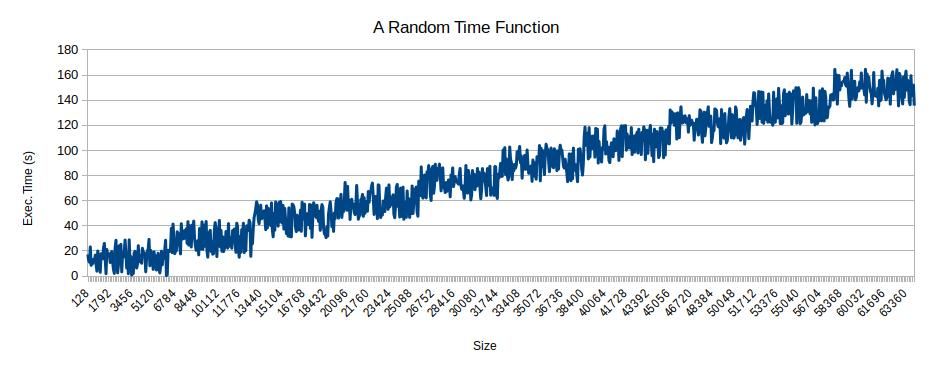
\includegraphics[width=6in]{Images/randonTimeFunction.jpg}
\caption{A random time function}
\label{fig:randomTimeFunction}
\end{figure}

\subsection{Parallel Execution Time Improvement}
Figure \ref{fig:etimeComp} compared the execution time of load-equal distribution with that of heterogeneous one for 16 processors. In this figure, horizontal and vertical axes show workload sizes and parallel execution times, respectively. Workload sizes rage from 1024 ($=16*64$) to 1024000 ($=16*64000$) with granularity of 64.

\begin{figure}[!t]
\centering
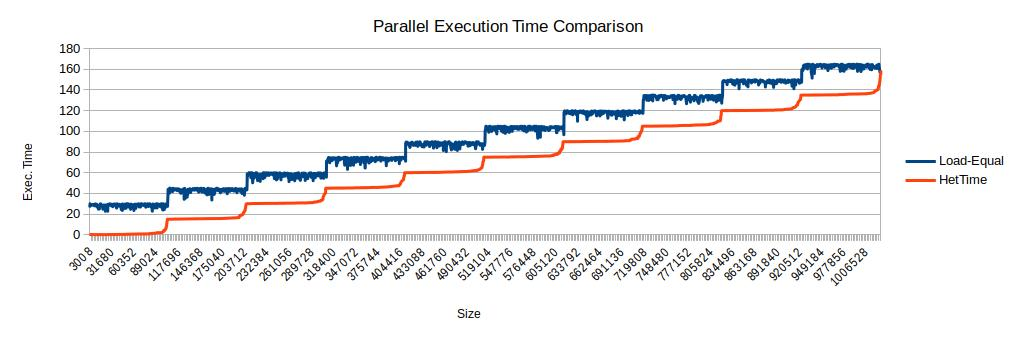
\includegraphics[width=6in]{Images/eTimeCompare_set16.jpg}
\caption{Load-equal vs. heterogeneous distribution}
\label{fig:etimeComp}
\end{figure}

\subsection{Processing Time}
In this section we are going to examine the processing speed of the proposed algorithm. Figures \ref{fig:pTime16} and \ref{fig:pTime128} show the time taken to find optimal solutions for 16 and 128 processors. Each time function consists of 1000 data points with granularity of 64. The experiments have been run on HCLServer.

\begin{figure}[!t]
\centering
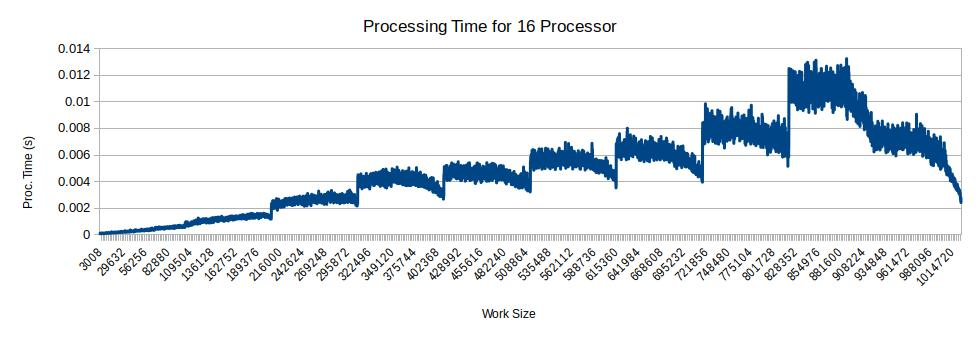
\includegraphics[width=6in]{Images/procTime_set16.jpg}
\caption{The time consumed to find optimal heterogeneous distributions for 16 processors.}
\label{fig:pTime16}
\end{figure}

\begin{figure}[!t]
\centering
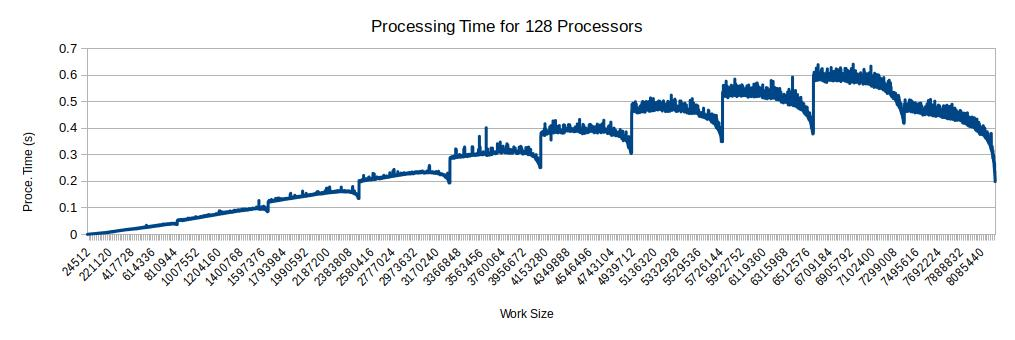
\includegraphics[width=6in]{Images/procTime_set128.jpg}
\caption{The time consumed to find optimal heterogeneous distributions for 128 processors.}
\label{fig:pTime128}
\end{figure}

\subsection{Time Complexity}
According to section \ref{sec_timeComp}, the proposed algorithm's processing time is bounded by $O(n * d * p)$. Since the number of maximum points in every time function ($d$) is not too large, it can be considered as a constant, and it means that the processing time will be a parameter of both work-size ($n$) and the number of processors ($p$). To evaluate the correctness, figures \ref{fig:n_p_time} and \ref{fig:n_p_recCall} depict how $n$ and $p$ affect processing time and the number of recursive calls, respectively. Work sizes range from 8192 to 256000, and the number of processors varies between 4 and 128. It is apparent that there is a linear relationship between both $n$ and $p$ with processing and recursion calls. 

\begin{figure}[!t]
\centering
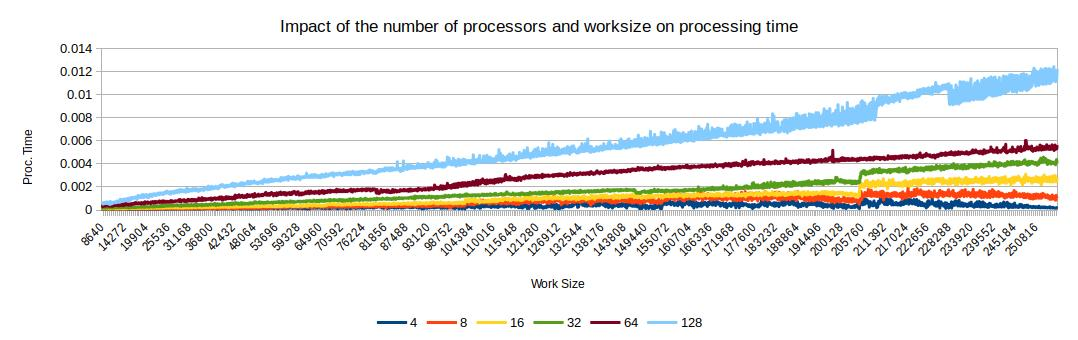
\includegraphics[width=6in]{Images/n_p_time.jpg}
\caption{The relationship of work-size and number of processors with processing time.}
\label{fig:n_p_time}
\end{figure}

\begin{figure}[!t]
\centering
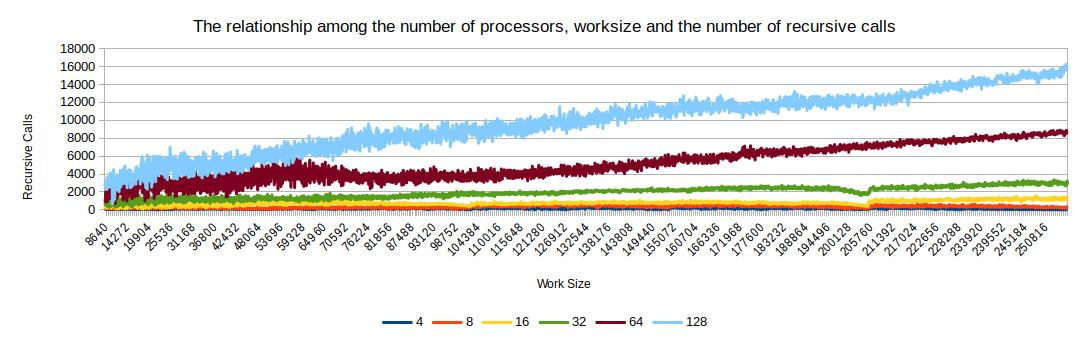
\includegraphics[width=6in]{Images/n_p_recCall.jpg}
\caption{The relationship of work-size and number of processors with recursion calls}
\label{fig:n_p_recCall}
\end{figure}

\end{document}